\documentclass[../BimodalReference.tex]{subfiles}
\begin{document}

\section{Introduction}

\textbf{TM} is a bimodal logic combining S5 a historical necessity operator ($\nec$) with linear temporal operators for past ($\allpast$) and future ($\allfuture$).
The logic provides a framework for reasoning about necessary truths across time to train AI systems to reason about past and future contingency.

The semantics is based on \emph{task frames}, which extend Kripke frames with temporal structure.
A task frame consists of world states connected by a \emph{task relation} indexed by temporal durations.
World histories are temporal slices through a task frame, representing the unfolding of a world over time.

\begin{center}
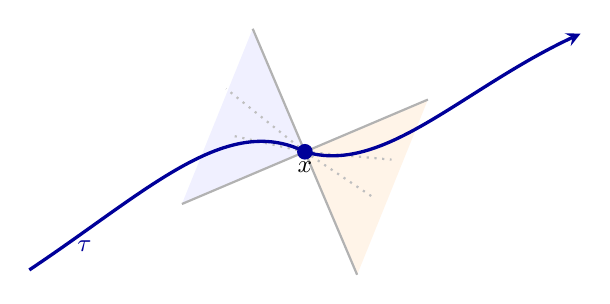
\begin{tikzpicture}[
  worldline/.style={very thick, blue!60!black},
  lightcone fill/.style={opacity=0.15},
  lightcone edge/.style={gray!60, thick},
  counterfactual/.style={dotted, thick, gray!50},
  point/.style={circle, fill=blue!60!black, inner sep=2pt}
]
  % Define the marked point P
  \coordinate (P) at (0,0);

  % Tangent direction at P: from control point (-1,0.5) toward (1,-0.3)
  % Direction vector (2,-0.8), angle = atan(-0.8/2) ≈ -22 degrees
  % Light cone size: 1.7 units (2/3 of original 2.5)

  % Future light cone (opens in direction of travel, rotated -22 degrees)
  \begin{scope}[rotate=-22]
    \fill[orange!60, lightcone fill] (P) -- (1.2,1.2) -- (1.2,-1.2) -- cycle;
    \draw[lightcone edge] (P) -- (1.2,1.2);
    \draw[lightcone edge] (P) -- (1.2,-1.2);
  \end{scope}

  % Past light cone (opens opposite to travel, rotated 158 degrees)
  \begin{scope}[rotate=158]
    \fill[blue!40, lightcone fill] (P) -- (1.2,1.2) -- (1.2,-1.2) -- cycle;
    \draw[lightcone edge] (P) -- (1.2,1.2);
    \draw[lightcone edge] (P) -- (1.2,-1.2);
  \end{scope}

  % Draw counterfactual paths within cones (rotated to match cone orientation)
  % Past paths (within past cone, heading back-left-up)
  \draw[counterfactual] (P) -- (-1.0,0.8);
  \draw[counterfactual] (P) -- (-0.9,0.2);

  % Future paths (within future cone, heading forward-right-down)
  \draw[counterfactual] (P) -- (1.1,-0.1);
  \draw[counterfactual] (P) -- (0.9,-0.6);

  % Draw the S-shaped main worldline (actual history)
  \draw[worldline, ->, >=stealth] (-3.5,-1.5)
    .. controls (-2,-0.5) and (-1,0.5) .. (P)
    .. controls (1,-0.3) and (2,0.8) .. (3.5,1.5);

  % Label tau near beginning of worldline (at 1/4 length)
  \node[font=\small, blue!60!black] at (-2.8,-1.2) {$\tau$};

  % Draw the marked point P on top
  \node[point] at (P) {};
  \node[below, font=\small] at (P) {$x$};

\end{tikzpicture}
\end{center}

\noindent
The diagram above illustrates the conceptual structure underlying TM logic.
The solid curve $\tau$ represents a single world history---a temporal sequence of states.
From any point $x$ along a history, the past and future light cones contain all states that are modally accessible.
The necessity operator $\nec$ quantifies over all histories passing through $x$, while the temporal operators $\allpast$ and $\allfuture$ quantify along the single actual history.
The dotted lines represent counterfactual paths: alternative pasts that could have led to $x$, and alternative futures that could unfold from $x$.

\subsection*{Project Structure}

The Lean 4 implementation is in the \texttt{Bimodal/} directory:
\begin{itemize}
  \item \texttt{Syntax/} -- Defines the formula language with 6 primitive constructors and derived operators.
  \textbf{Complete.}
  \item \texttt{ProofSystem/} -- Axioms (14 schemata) and inference rules (7 rules) forming a Hilbert-style proof system.
  \textbf{Complete.}
  \item \texttt{Semantics/} -- Task frames model possible worlds; world histories model time; truth conditions define meaning.
  \textbf{Complete.}
  \item \texttt{Metalogic/} -- Soundness theorem (proven: all axioms valid, rules preserve validity), deduction theorem (proven: enables assumption introduction), and completeness infrastructure (Lindenbaum lemma, canonical model axiomatized).
  \textbf{Soundness and deduction complete; completeness pending.}
  \item \texttt{Theorems/} -- Perpetuity principles and modal theorems derived from the axiom system.
  \textbf{Partial.}
\end{itemize}

\end{document}
